
\chapter[LLM 训练流水线]{大语言模型训练流水线}\label{chap:pipeline}


\begin{learningbox}
在本章中，你将学习语言模型是如何训练的。具体来说，你将能够：
\begin{itemize}[leftmargin=*, nosep]
    \item 描述一个基础训练流水线的主要阶段，并说明各阶段的目的：{\em 数据获取、预训练、微调、偏好调优与推理}。
    \item 区分{\em 预训练与微调}，并解释为什么偏好调优要放在它们之后、而不是之前。
    \item 解释{\em 编码器/解码器}之分如何决定一个模型采用哪种训练目标。
    \item 识别用于评估语言模型的常见{\em 基准测试}，并说明每一项旨在衡量什么能力。
\end{itemize}
\end{learningbox}

\begin{comment}
In the previous chapter we have introduced the basic conceptual and technical elements of language modeling. These elements form the foundation of current language models. In this chapter, we will have a detailed look at how the models are trained by providing an overview of a typical training pipeline of LLMs. This includes the relevant \emph{pretraining} and \emph{posttraining} methods of standard (non-agentic) models. Note that later, in Chapter~\ref{chap:agents}, we will see further training methods, such as an agentic \emph{harness}, that will build on the training methods that we discuss in this chapter.  

Modern language models are large neural networks that are constructed with transformer blocks.
The transformer architecture uses the attention mechanism \citep{vaswani2017attention} to model connections between tokens, which ultimately yields versatile models for a wide range of tasks. But how do we construct these models and how might such language models be trained? 


In the remainder of this chapter, we discuss various types of models (Section~\ref{sec:pipeline-models}), the individual training pipeline stages (Section~\ref{sec:pipeline-training}), and how to measure whether your trained model actually is useful through stratified testing (Section~\ref{sec:pipeline-benchmarks}).
\end{comment}

\section{训练模型}

大语言模型的训练流水线遵循一套大致标准的方法：从一个参数随机初始化的模型架构出发，我们通过一个称为{\em 预训练}的过程训练出语言能力。在预训练中，我们把大规模文本语料喂给模型，以自回归方式训练它。这一阶段的产物是一个基础模型，它通常还不能直接用于具体的实际应用。因此，我们需要让它适配某个下游任务或用途。这一阶段称为{\em 后训练}，我们向模型展示特定类型的额外数据，借此激发任务特定的行为，例如指令遵循或分类任务。

\subsection{编码器模型与解码器模型}
如上一章所见，存在两种占主导地位的模型风格。一方面，编码器模型能够基于输入数据生成丰富的语境化表示。然而，近年来的多数成功都建立在解码器模型之上。编码器更擅长理解类任务（分类、情感），解码器则在生成类任务上表现出色。解码器模型的规模不断增长，无论是可训练参数数量还是可用的训练数据。这带来了泛化能力惊人的模型，能够应对未见过的语境。

下面我们更仔细地看一看解码器专用训练流水线中%Now that we have discussed the model's architecture, focusing on a decoder only, the next step is to dive into the 
相关的各个步骤。


\subsection{预训练/微调范式}


当前训练流水线取得成功的一个核心特征，是运用了迁移学习。现代 Transformer 模型的典型用法之一，是取一个已在大规模通用数据集上训练过的模型，再把它重新训练到一个新任务上。模型先在大规模通用语料上被{\em 预训练}，然后在新任务上被{\em 微调}——新任务通常只有一个小数据集。面向新任务的微调很快，因为数据集小，也因为预训练权重已被迁移过来，微调训练不必从零开始。

%In the pretraining phase, generic knowledge is encoded in the weights of the model. Finetuning on the smaller dataset is quicker, and by making the distinction between pretraining and finetuning, models can be created quickly that perform well on specific tasks. The pretrained weights are reused (transferred) to jump start the training in the finetuning phase. 

这种迁移学习范式中「预训练/微调」的区分，正是大语言模型训练流水线的核心。
模型不必从零开始训练，而是可以在新场景中复用已经学到的语言知识，从而加快训练过程。大型商业模型的预训练可能耗时数月。通常，新任务是具体的（例如某一领域的问答，或情感分析）。针对新任务，会用一个专门的数据集来微调模型。在微调过程中，模型的一部分权重被小心地更新，以保留预训练模型的一般语言能力，同时获得对新任务的理解。把一个模型微调到新任务上，通常只需几分钟到几小时。


\subsection{开放模型与闭源模型} 
\label{sec:pipeline-models}
流行的 LLM 包括 OpenAI 的 ChatGPT 系列 \citep{achiam2023gpt,ouyang2022training}、Meta 的 LLaMa 家族 \citep{touvron2023llama}、Google 的 Gemma \citep{chowdhery2023palm} 与 Gemini
\citep{team2023gemini}、Anthropic 的 Claude 家族、Moonshot AI 的 Kimi、DeepSeek \citep{guo2025deepseek} 以及 Qwen \citep{bai2025qwen2} 等等。

这些模型的开放程度各不相同。例如，模型的训练数据可以公开，模型的网络架构可以披露，训练好的权重可以发布。然而，商业模型背后的公司很少公布其模型与训练流程的全部要素，因为它们希望保留一定的竞争优势。

作为回应，科学界发展出了完全开源的模型，例如 BLOOM \citep{le2023bloom}、Pythia \citep{biderman2023pythia} 与 OLMo \citep{groeneveld2024olmoacceleratingsciencelanguage}，以推动对大语言模型工作原理的集体理解。这些模型的训练流水线各要素全部公开，也是本章关注的焦点。我们也会指出一些商业模型的某些方面。

尽管这些模型都基于 Transformer 架构，但各组件及其整体布局之间存在细微差异，例如为了利用硬件差异，或采用各自开发者研发的特定优化。举例来说，Google 为其基于 TPU 的计算基础设施对 Gemini 做了优化 \citep{jouppi2023tpu}。关于架构的进一步改进，%, specifically those aimed at optimizing the model (either in terms of memory or throughput) 
我们在第~\ref{chap:scaling} 章中有大量讨论。


%As pretraining data increases in size (often a considerable ratio of the total size of the internet), the line between in- and out-of-domain data becomes increasingly blurred, especially given that commercial vendors often do not specify the sources of their training data (either out of commercial interest or for other  reasons). Hence, when we wish to measure true generalization to unseen data,  we need to take measures to ensure that the model has not seen the data before (we wish to prevent {\em data contamination}).  

\section{训练流水线}
\label{sec:pipeline-training}
下面我们更详细地描述一个标准训练流水线的各个步骤。
LLM 是借助一条包含不同训练阶段的精细流水线构建出来的 \citep{radford2019language,minaee2024large}。我们将描述这些阶段，如图~\ref{fig:llm-training-pipeline} 所示。各阶段的组合通常被称为训练{\em 配方}（recipe），因为它们指明了模型按何种顺序被训练。每个阶段可能使用新的数据集，配合新的损失函数。每个阶段的目的都是赋予模型某一项特定能力。随着我们逐一讨论各阶段，这一点会变得清晰。



\begin{figure}
    \centering
    \includestandalone[width=\textwidth]{part1/visuals/tikz/llm_pipeline_overview}
    \caption{LLM 训练流水线概览 \citep{radford2019language,minaee2024large}。}
    \label{fig:llm-training-pipeline}
\end{figure}

\subsection{获取数据}
流水线的第一步是获取数据。通常使用大规模通用文本语料 \citep{brown2020language}。这些语料由无需人工标注的原始文本构成。这类数据一般汇集自经过筛选与未经过筛选的在线来源，再通过清洗启发式规则加以提纯，以减轻有害、隐私或受版权保护内容的影响。
%
用于预训练的语料规模巨大。现代 LLM 是在网络级规模的数据上训练的，常常达到数万亿词元的量级。数据集的一些例子有：

\begin{itemize}
    \item Common Crawl：一个庞大的、非营利的网络快照，包含数十亿个页面；替代来源包括 \url{https://archive.org}。其规模无与伦比，但数据质量仍有争议 \citep{baack2024critical}。许多衍生物，如 C4（Colossal Clean Crawled Corpus，巨型清洁爬取语料），提供了英文网页文本的过滤子集 \citep{raffel2020exploringc4}，以提升数据质量。
    \item Dolma 3：一种数据混合，旨在最大化在一系列多样任务上的性能。它被用于 OLMo 开源/开放数据项目 \citep{olmo2025olmo3, soldaini2024dolma}。
    \item SmolLM3：采用大规模的三阶段训练策略，使用 11.2 万亿词元，动态混合网页、数学与代码数据，以优化推理与知识获取 \citep{bakouch2025smollm3}。
\end{itemize}
%
近期研究强调，对于提升跨领域知识与下游泛化而言，数据多样性之重要不亚于规模 \citep{gao2020pile800gbdatasetdiverse}。名为 {\em The Pile} 的语料就是专门作为异构语料构建的。例如，在 The Pile 上训练的模型在编码效率（每字节比特数，Bits Per Byte，BPB）\footnote{每字节比特数是一个与分词器无关的信息论指标，衡量平均每个符号所需的比特数，反映编码效率，另见第~\ref{sec:metrics} 节。}上，在 GitHub 仓库、医学论文、哲学文本等差异很大的领域中都表现出显著提升（见图~\ref{fig:pile}）。因此它常被用作基准测试——在 Pile BPB 上的良好表现，可作为模型世界知识与复杂推理能力的指标。

为预训练整理数据，需要定义复杂的数据清洗流水线，把来自多个来源的原始数据转化为一个干净的纯文本文档集合。这一过程往往聚焦于质量保证与安全性。整理过程始于来源优先级排序，即让数据混合向高质量来源倾斜，例如维基百科、书籍以及其他已知的经筛选来源。此外，为确保语料的一致性，研究者会应用降噪启发式规则，剔除模板化文本、导航菜单以及可能不当的内容。还会在 URL 与文档两个层级做去重；这对于防止模型记忆冗余信息、在重复数据上过拟合至关重要。

除准确性之外，流水线还必须筛选符合安全与伦理约束的数据。这同样通常通过基于启发式规则的过滤来实现。此外还会部署毒性检测系统来移除仇恨言论，尽管这些方法的结果往往参差不齐。这一阶段的一大挑战是偏见缓解：自动过滤器可能无意中把用特定方言（例如非裔美国人英语）写成的合法数据标记为问题并加以压制，从而把多元的声音意外排除在训练集之外。

\begin{figure}[tb]
    \centering
    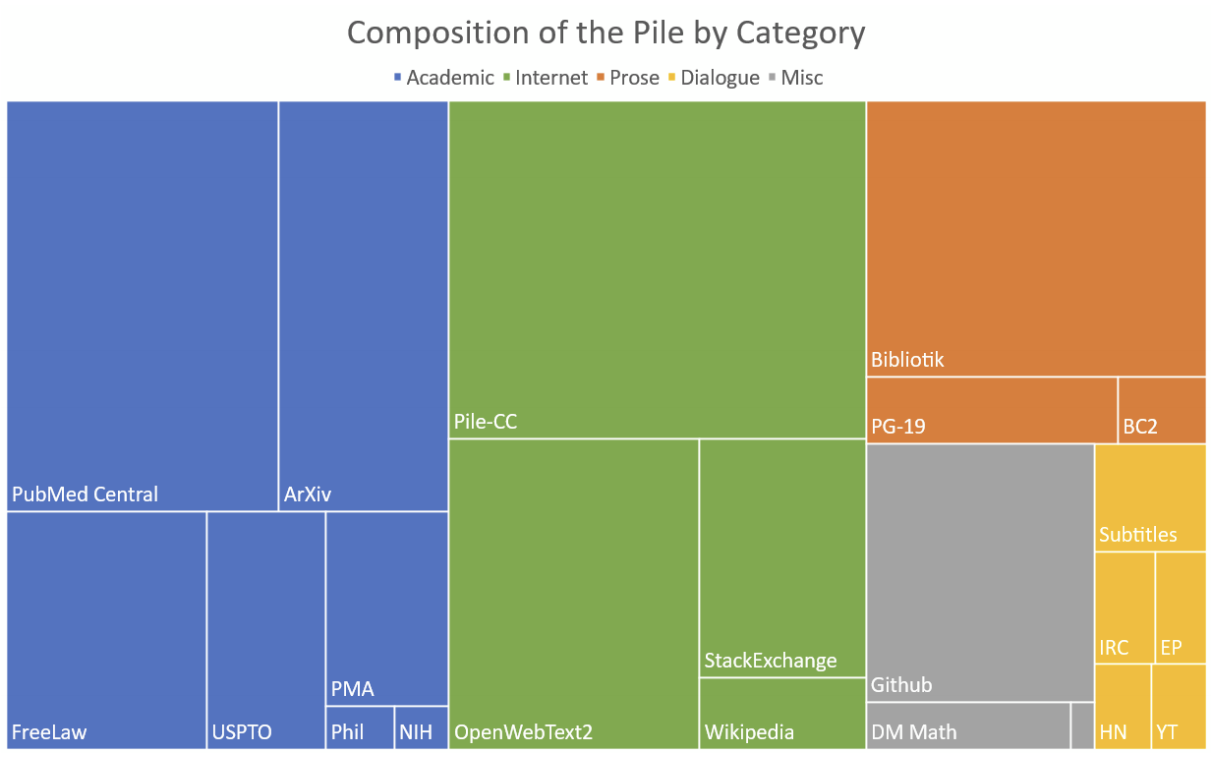
\includegraphics[width=0.9\linewidth]{part1/visuals/the_pile.png}
    \caption{The Pile 数据集内部数据来源概览 \citep{gao2020pile800gbdatasetdiverse}。}
    \label{fig:pile}
\end{figure}


\subsection{预训练}
训练流水线的第二步是在整理好的语料上预训练模型，这一过程产出一个通用型自然语言模型。该阶段在无标注文本上使用自监督的 Transformer 方法 \citep{vaswani2017attention}。

为了获得语言的内部表示、概念的语义关系与世界知识，模型以掩码词元填空式任务来训练。
%---where the model must iteratively predict masked tokens conditioned on a preceding context---the architecture develops .
%
在这类任务中，%Pretraining of LLMs is done using cloze-like tasks, in which 
目标是：在由大规模序列语料（即文本、图像块的表示）构成的给定前文语境条件下，预测被掩码的词元。这一过程是自监督的（不需要人工标注数据），已知能够产出丰富的语言表示、概念之间的关系以及各种形式的世界知识。

形式上，语言建模目标是在给定已有词元的窗口 $k$ 的条件下，最大化句子 $\mathcal{U} = \{u_{0}, \dots, u_{n} \}$ 中词元的概率（式~\ref{eq:lm}）。$L(\mathcal{U})$ 就是{\em 语言建模损失}。

\begin{equation}
\label{eq:lm}   
    L(\mathcal{U}) = \sum_i \log P(u_i | u_{i-k}, \dots, u_{i-1}; \Theta)
\end{equation}

语言模型通过可训练参数 $\Theta$ 来估计这些概率，并以梯度更新进行优化。鉴于模型规模从数百万到超过一万亿参数不等，要保证收敛就需要大规模数据集。在这一训练阶段，会采用教师强制：模型做出一个预测，但提供给下一步的输入是真实词元，而不是模型自己的输出。相比之下，在推理时的自回归生成中，模型必须把自己此前的预测作为后续词元的输入。词元由运行相应的{\em 分词器}产生，详见第~\ref{sec:tokenization} 节。

在预训练中，一个关键挑战是确保模型在数万亿次梯度更新中高效学习并保持稳定。随着时间推移，人们发展出多种旨在让训练过程保持可控的策略。其中之一是课程学习。在人类学习中，我们先学容易的概念（例如加法），再去攻克更难的概念（乘法、对数）。在语言建模中，这一思想被用于数据混合，即数据课程。研究者不是同时训练所有类型的数据，而是先选定一种特定的数据来源混合来训练，示例见图~\ref{fig:smollm3-mixture}。构造混合涉及按难度对数据做策略性排序。在一套训练课程中，我们先从易于学习的通用网页爬取数据入手，再在后续阶段转向更难的高质量推理数据（数学与代码）。其基本想法是，这有助于模型更快地在更复杂的逻辑上收敛 \citep{bengio2009curriculum}。

\begin{figure}[tb]
    \centering
    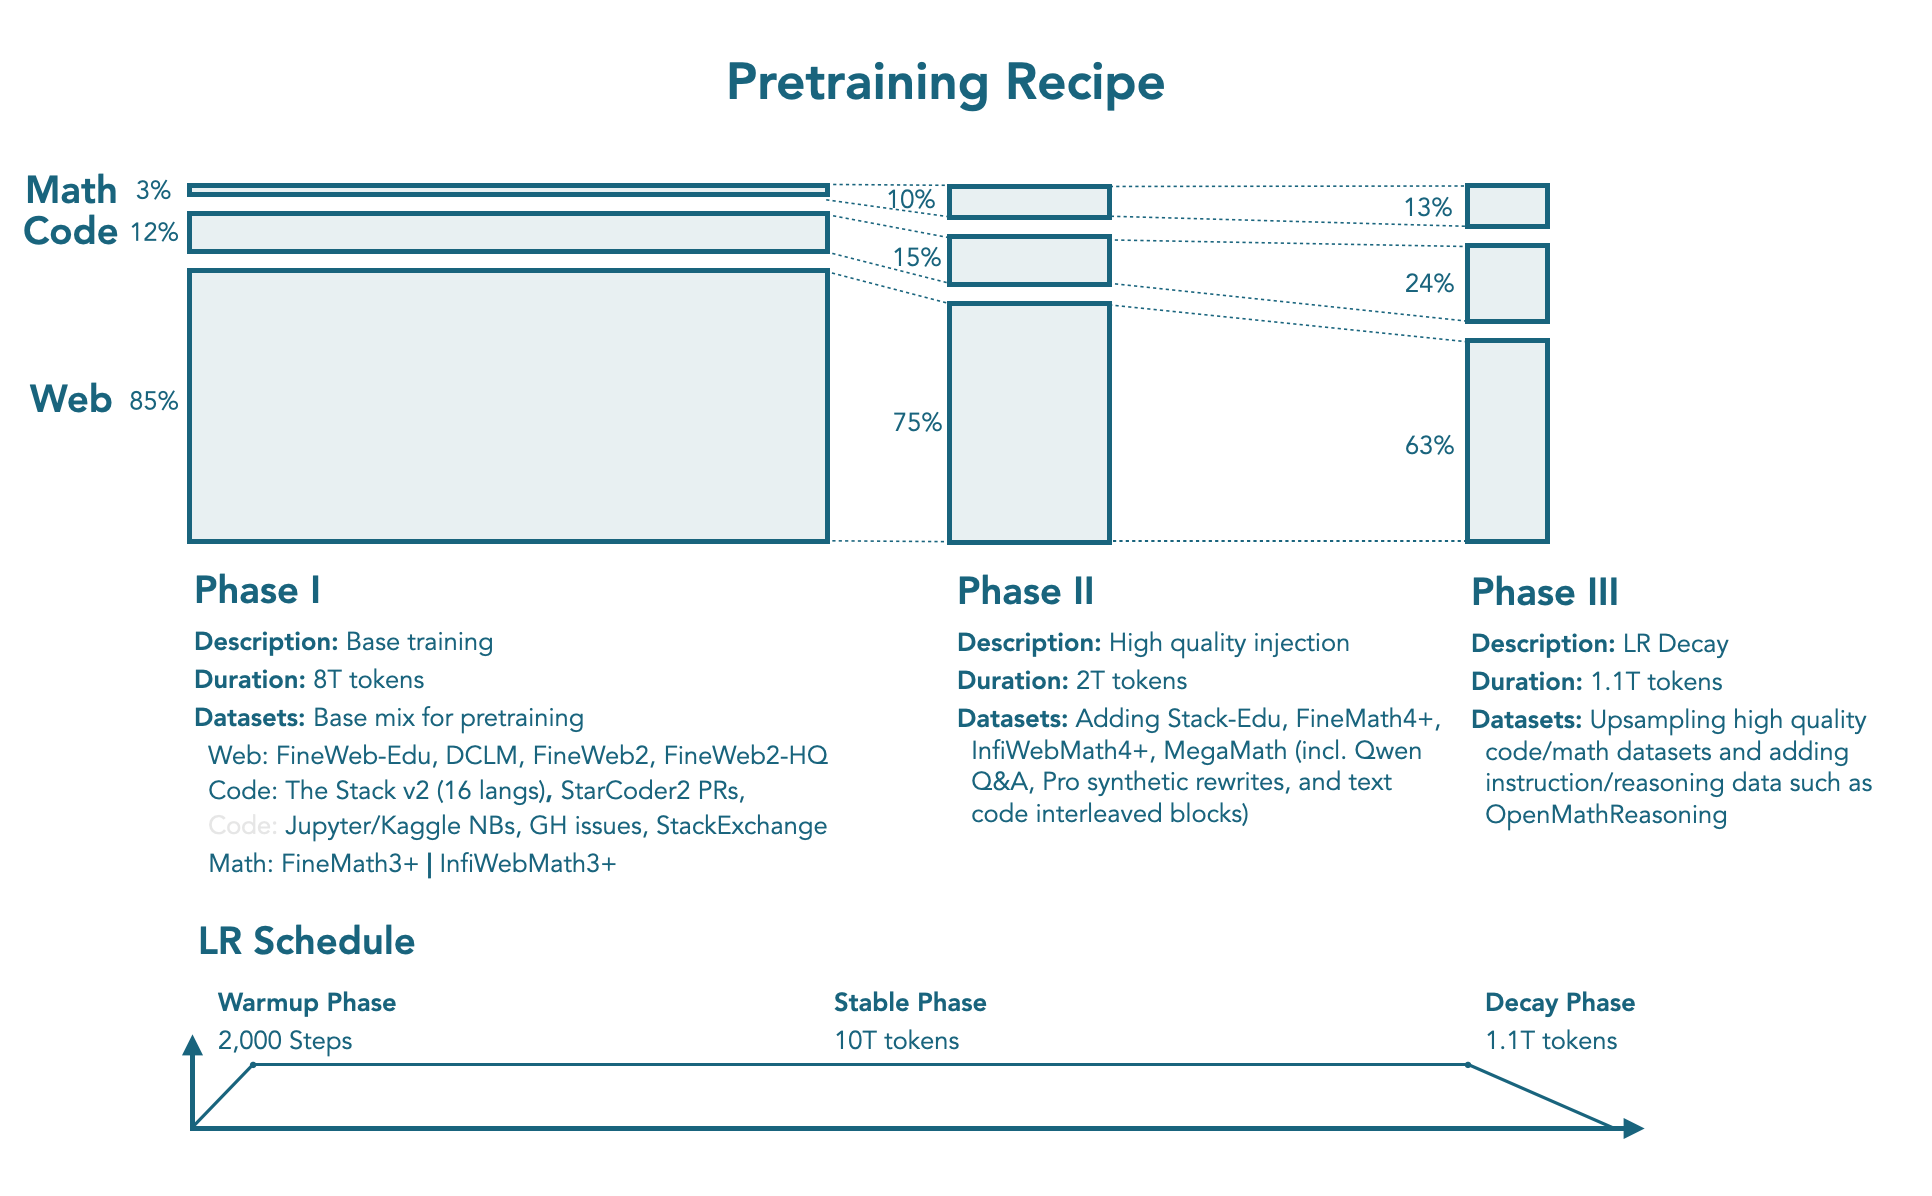
\includegraphics[width=0.75\linewidth]{part1/visuals/smollm3_mixture.png}
    \caption{训练 SmolLM3 所用的数据混合示例 \citep{bakouch2025smollm3}。}
    \label{fig:smollm3-mixture}
\end{figure}

人们还采用其他稳定训练的机制，因为在这一规模上的训练以不稳定著称，容易出现损失尖峰 \citep{takase2025spikemorestabilizingpretraining}。稳定性通过标准的机器学习技术来维持，例如权重衰减、层归一化以及精巧的学习率调度器。使用专门的优化器并监控梯度范数，有助于防止参数在密集的预训练过程中发散。图~\ref{fig:glm-spike} 给出了一个例子，说明更换嵌入层如何带来更稳定的训练。左图展示了 336M 与 752M 参数 BERT 模型的训练损失。原始架构在 336M 模型上表现良好，而 (b) 中的改动则使训练更稳定、训练损失更低 \citep{shoeybi2020megatronlmtrainingmultibillionparameter}。

\begin{figure}[tb]
    \centering
    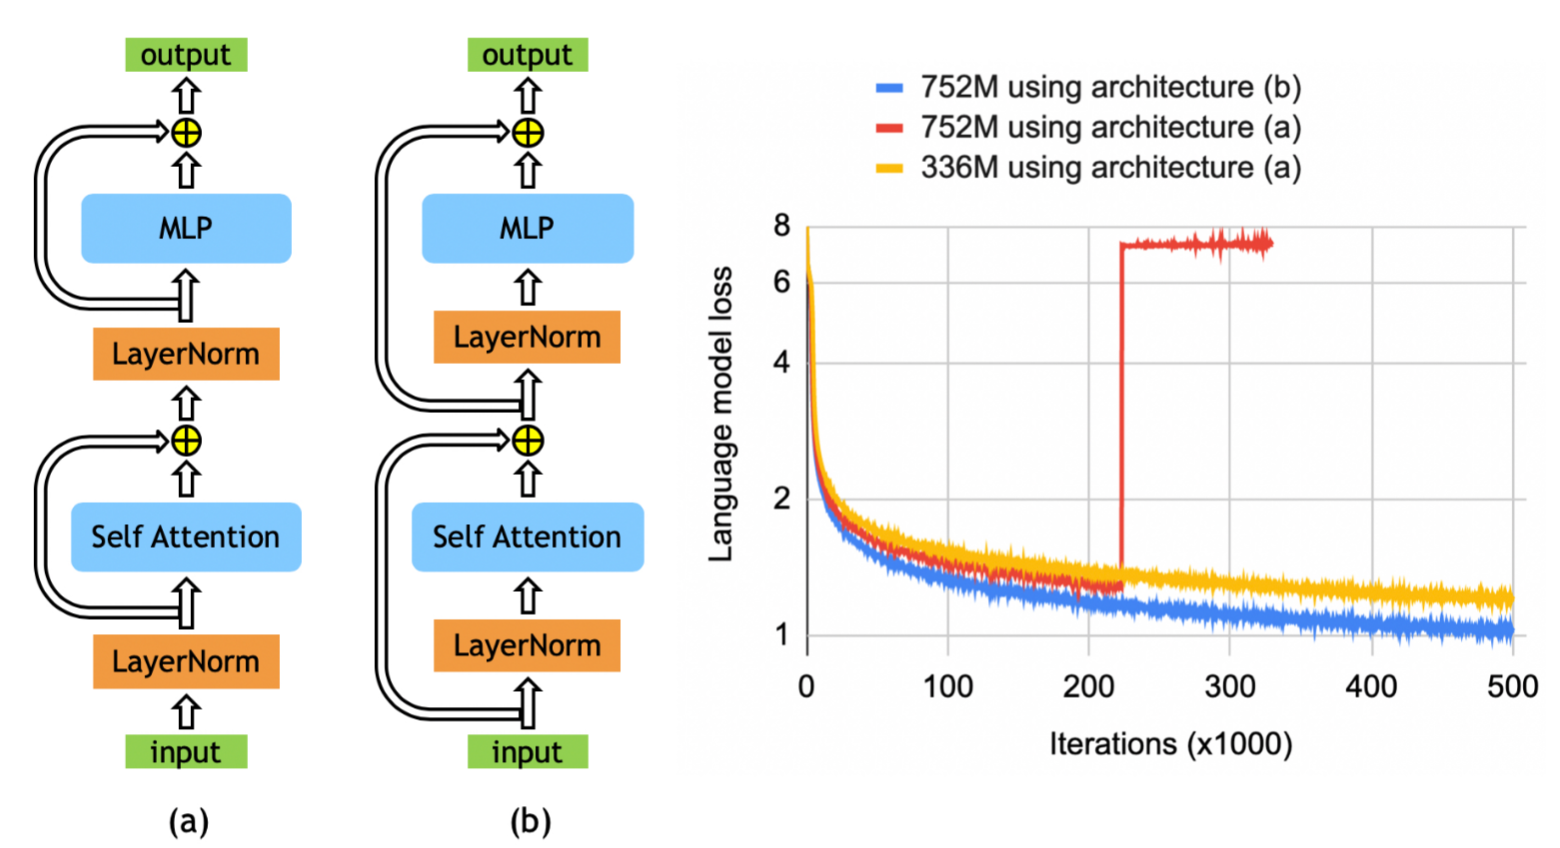
\includegraphics[width=0.75\linewidth]{part1/visuals/glm_spike.png}
    \caption{采用原始架构 (a) 与重排架构 (b) 的 BERT 模型训练损失 \citep{shoeybi2020megatronlmtrainingmultibillionparameter}
    }
    \label{fig:glm-spike}
\end{figure}


\subsection{微调}
预训练之后是后训练，其中第一个重要的训练步骤是微调。
LLM 很少被用在「自动补全式的通用下一个词预测」场景中；人们更多是用它们来回答问题、给出建议和回忆信息。微调是指：取一个已经学会一般语言模式的预训练模型，再在一个更小、更具体的数据集上继续训练它。在微调中，我们用监督学习的方法，把一个通用模型应用到一个有标注数据集上的具体（狭窄）任务。
一种流行的高效方法是低秩优化，它只微调一小部分参数 \citep{hu2021lora,wei2022emergent,minaee2024large}。

\paragraph{监督微调（SFT）}
微调可以应用于许多专门任务。最通用的模型会使用{\em 监督微调}，以获得遵循指令和执行推理步骤的能力 \citep{olmo2025olmo3}。监督微调这一步对较小的模型尤其重要，它提供了一种高效机制，能显著提升通用对话、推理与函数调用能力。


监督微调也被用于更专门的任务，例如降低毒性。WildChat \citep{zhao2024wildchat} 提供了超过一百万条真实用户与 ChatGPT 的交互，记录了人类以各种复杂度与毒性水平向 LLM 提问的方式。

为学习推理能力，OpenThoughts \citep{guha2025openthoughts} 包含了逐步推理链，它们从高级模型中蒸馏而来，用于增强数学、科学与编程方面的解题能力。人工获取的数据由合成数据补充——即用更大的教师模型（如 GPT-5）生成指令与回答，以填补特定的数据空缺并扩大训练量 \citep{zhang2026instruction}。
 
%\paragraph{Other tasks}
微调并不只关乎通用的指令遵循或推理。其他任务可以是例如语言之间的翻译，或医疗、客服领域的问答。尤其对于任务狭窄、模型较小的工业应用而言，微调是一项颇有成效的工作。

在第~\ref{sec:tools} 章中，我们将讨论 LLM 对工具的使用，这是智能体大语言模型的一个核心方面。使用工具的训练同样发生在训练流水线的监督微调步骤中
\citep{wei2022emergent,minaee2024large}。


此外，微调对于确立模型的人格形象、加深其专业能力也很有帮助。例如，机构可以训练模型采用特定的语气，让客服机器人保持一致的品牌形象——无论是富有同理心且正式，还是机智而随性。最后，注入深度领域知识能让模型掌握小众领域的繁复术语与逻辑，例如行业特定的专利信息，或调试专有的遗留代码。

归根结底，微调把一个通用预测器转变为专门的专家，常常使更小、更高效的模型在特定任务上超越更大的基础模型。


\subsection{偏好调优}
早期模型暴露出一个问题：训练往往会放大训练数据中极端、社会不可接受的文本，并任其泛滥，从而挤占温和的观点。自那以后，让 LLM 变得社会可接受的一个关键步骤，就是在流水线中加入一个阶段，把模型调校为以社会可接受的方式行事。这一阶段称为偏好调优。

在这一阶段，我们让微调后的模型与用户预期对齐（偏好对齐）。这一步的目标是改进模型，使其给出社会可接受的回答、防止仇恨言论、减少幻觉并提升指令遵循度。

偏好调优的标准方法包括基于人类反馈的强化学习（RLHF）\citep{ouyang2022training}——它训练一个奖励模型来逼近人类价值观；以及直接偏好优化（DPO）\citep{rafailov2024direct}——它直接从偏好数据中优化策略。RLHF 的高层概览见图~\ref{fig:rlhf-loop}。为解决人工标注这一瓶颈，现代流水线越来越多地采用基于 AI 反馈的强化学习（RLAIF）\citep{bai2022constitutional}，由更强的模型来生成偏好信号。

\begin{figure}[tb]
    \centering
    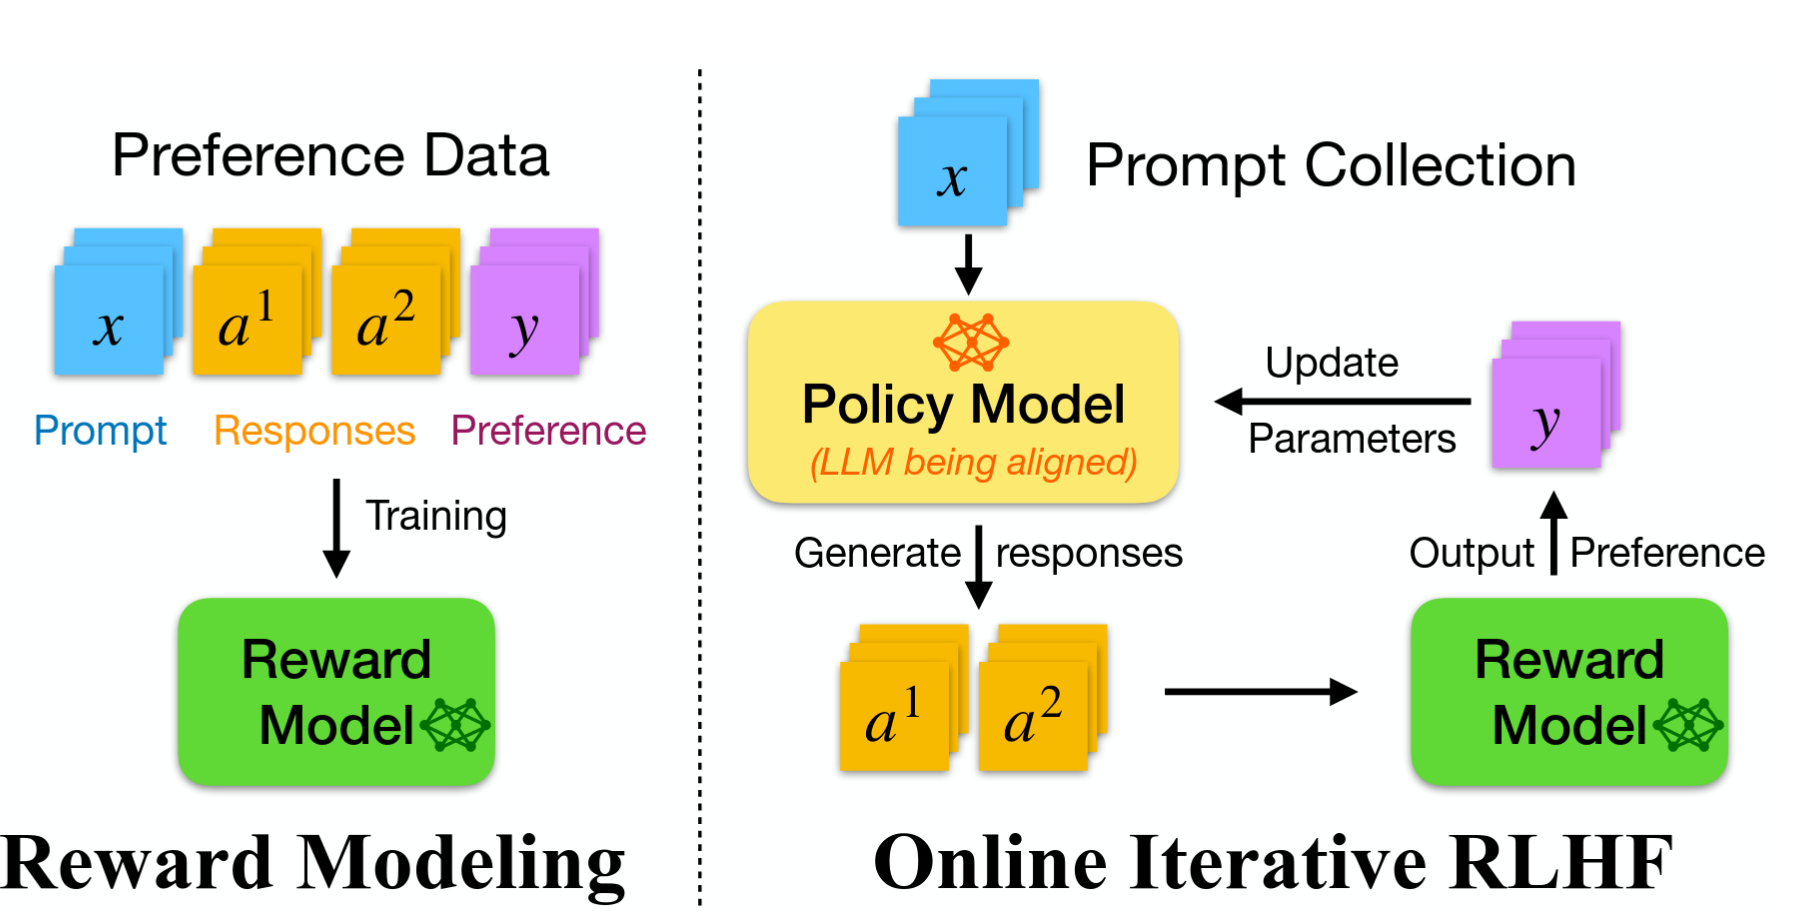
\includegraphics[width=0.5\linewidth]{part1/visuals/rlhf_loop.png}
    \caption{RLHF 高层概览：训练一个奖励模型（左），并针对该奖励模型优化语言模型（即策略）\citet{dong2024rlhf}}
    \label{fig:rlhf-loop}
\end{figure}

与人类价值观对齐并非易事，我们通常区分安全对齐、价值对齐与偏好对齐。在最后一种情形中，一个麻烦在于偏好是主观的（例如写作风格），因人而异。

\paragraph{价值对齐}
在更高层面上，价值对齐关注的是确保模型的底层原则与世界观与广泛的人类伦理相契合。与个人偏好不同，这涉及把模型锚定在公平、有用、诚实等高层概念上。在实践中，这意味着模型受一套成文原则（{\em 宪法}）约束，以确保它遵守开发者制定的政策。
% alignment tax

然而，这种价值对齐通常会带来取舍：为安全性与有用性而优化模型，也会削弱它在其他能力上的表现，例如事实回忆或创造力 \citep{lin2024mitigating}。这种取舍也被称为{\em 对齐税}。


\paragraph{安全对齐}
安全对齐是对模型行为设定硬边界，以防止灾难性或有害输出的过程。偏好对齐可能关注语气，价值对齐关注观点，而安全对齐关注对抗鲁棒性与拒绝恶意提示。确保安全的方法示例包括红队测试——让模型经受严苛的越狱尝试以发现漏洞；以及护栏——为高风险回答过滤出明确的拒绝边界。

\paragraph{目标对齐}
最后，对于存在客观真理的领域（如数学或编程），人们采用称为可验证奖励强化学习（RLVR）\citep{lambert2024tulu} 的方法。与标准 RLHF 不同，RLVR 通过利用真实信号来优化客观正确性，从而稳健地提升推理能力。例子包括能通过编译的代码，或正确的数学解答。在后一种情形中，常使用组相对策略优化（GRPO）算法 \citep{guo2025deepseek}——它是近端策略优化（PPO）的一个变体，在增强数学推理能力的同时也优化 PPO 的显存占用。其做法是从策略模型采样多个答案，用它们的相对质量（由验证器评定）来计算奖励。模型不再依赖人工标签来判断什么算好答案，而是从确定性验证器那里获得直接奖励（+1 或 -1）\citep{guo2025deepseek, shao2024deepseekmath}，见图~\ref{fig:grpo}。

\begin{figure}[tb]
    \centering
    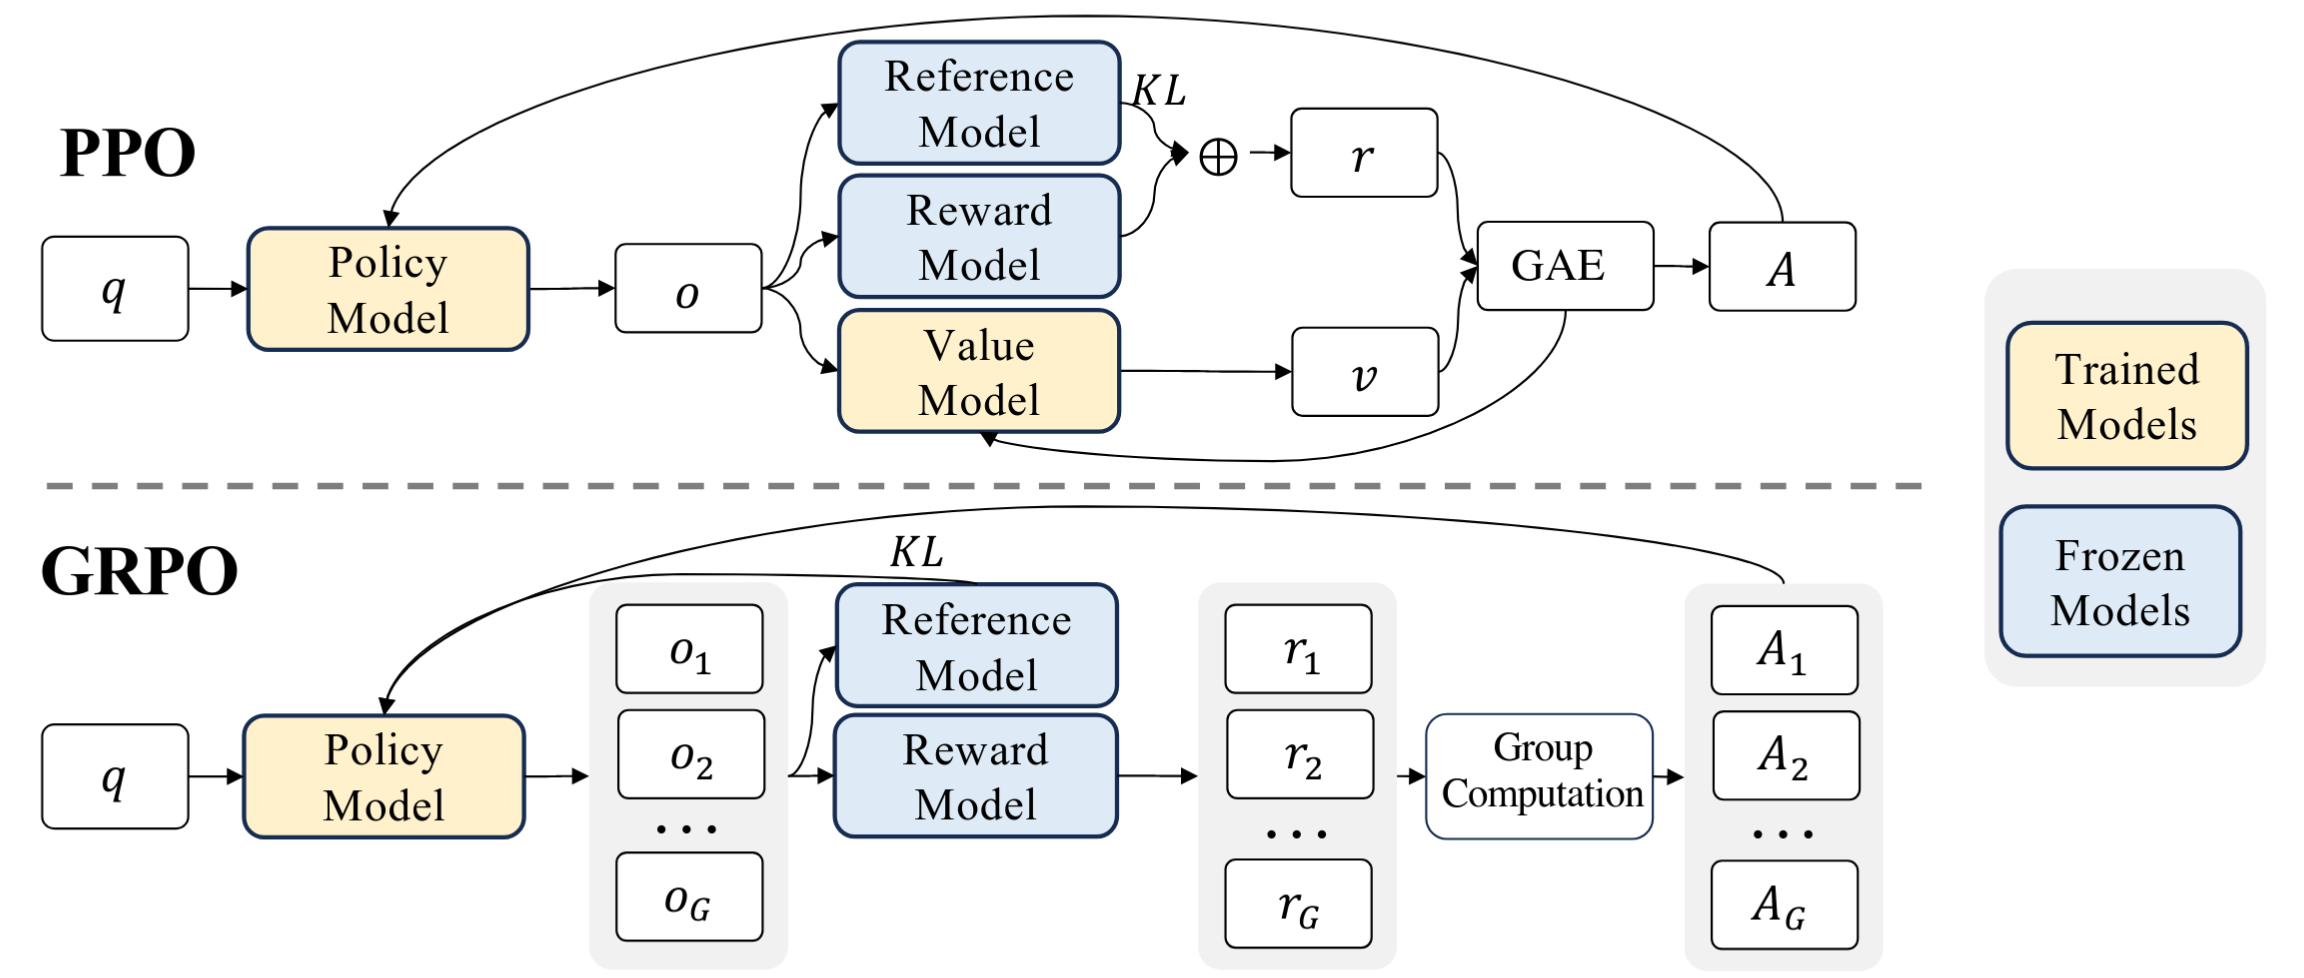
\includegraphics[width=0.8\linewidth]{part1/visuals/grpo.png}
    \caption{RLHF（具体为 PPO）与 RLVR（具体为 GRPO）方法的对比 \citep{shao2024deepseekmath}}
    \label{fig:grpo}
\end{figure}

\subsection{推理}
训练流水线的最后一步是推理步骤。这是最终使用训练好的模型的步骤。
在这里，用户终于能与模型交互。我们终于可以享用训练努力结出的果实。

在推理时，我们用自然语言提示词（指令与问题）从模型获取回答。提示是使用 LLM 让模型回答我们问题的首选方式。推理结果可能对提示词的表述方式很敏感。使用某些词，或调整提示词中词语的顺序，都可能影响模型的回答。这种敏感性催生了提示词工程与上下文工程——这些技能对 LLM 使用者而言已变得很重要 \citep{sahoo2024systematic}。

有意思的是，正如上一章所讨论的，在规模超过数千亿参数的解码器模型中，一种新的学习方法涌现出来：{\em 上下文学习}（ICL）\citep{brown2020language,wei2022emergent}。上下文学习是一种在提示词中包含少量示例并附上指令的方法。这些示例把模型引向某个方向，模型用它们来学会答案。ICL 是提示词内少样本学习的一种形式。ICL 也是一种不改变模型任何参数的学习——它是不经参数训练的示例学习 \citep{dong2022survey}。%Examples of ICL are zero-shot, one-shot, and then few-shot prompting, providing zero, one, and a couple examples for each inference. 

在本书余下部分，我们将看到许多使用上下文学习方式的例子，例如在智能体运行框架中。推理时的上下文学习是智能体大语言模型的一大驱动力。

\subsection{结语}
至此我们描述了典型 LLM 训练流水线的各个阶段。
请注意，我们描述的流水线只是典型做法的一个例子，不同模型的训练方式各不相同。当前的现代训练流水线十分精细，训练成本高昂。对训练流水线的创新是当前研究的课题，例如可参见 \citet{guo2025deepseek,team2025kimi}。

能够快速得到预测结果至关重要，人们已发展出多种技术来加速这一过程。例如，在推理投入与回答质量之间取得平衡很重要。对{\em 测试时缩放}的研究正是在考察这一取舍。推理时投入越大，消耗的计算时间越多，但可能得到更好的答案。我们将在第~\ref{chap:scaling} 章讨论这些以及其他优化技术。


\section{基准测试与性能}
\label{sec:pipeline-benchmarks}
在流水线训练出模型之后，我们希望弄清模型表现如何。
LLM 是用各种各样的建模技术、面向不同任务、在不同数据集上构建出来的。因此，它们往往获得了非凡的能力。例如，LLM 在自然语言理解任务（GLUE、SQUAD、Xsum）\citep{wang2018glue,wang2019superglue,rajpurkar2016squad,narayan2018don}、翻译 \citep{kocmi2022findings,papineni2002bleu,sennrich2015improving}、问答任务 \citep{roberts2020much} 以及诗歌创作 \citep{zhang2024llm} 上都表现出色，这里仅举几个领域。LLM 的广泛适用性体现了它们的多才多艺，尽管该领域的快速发展以及持续的研究努力，也提出了许多关于 LLM 在许多领域与语境中能力的开放问题。

下面我们讨论常用于测试模型性能的基准测试。

\subsection{常见任务}
让我们更仔细地看看一些常见的 LLM 任务。这些任务大体上可归入我们此前介绍过的两大语言处理类别：自然语言理解（NLU）与自然语言生成（NLG）。
取决于类别、任务的具体表述以及底层数据，性能指标会有所不同。我们分别讨论。

请注意，{\em 性能}是一个含义模糊的词。在自然语言处理中，它常指\emph{任务性能}（准确率），而不是\emph{计算性能}（速度）。尽管确切的评估标准因任务而异，现代评估实践主要关注任务性能。然而，我们向 LLM 发起多少次调用、能多快得到模型的回答，对于在当代基准测试上取得高分同样重要，我们将在后面几章看到这一点。


\subsection{指标}\label{sec:metrics}
为了监测或报告 LLM 的（任务）性能，我们会根据所处的训练阶段使用不同的指标。

\paragraph{预训练指标}
在预训练中，我们主要关心模型能否准确预测下一个词。标准指标是{\em 困惑度}，如式~\ref{eq:perplexity} 所示。困惑度衡量模型在预测下一个词元时的不确定性，与交叉熵损失函数直接相关。困惑度低，说明模型给正确的下一个词元分配了高概率。对困惑度而言，越低越好。

\begin{equation}
    \text{PPL}(X) = \exp \left( - \frac{1}{N} \sum_{i=1}^N \log P(x_i \mid x_{<i}) \right)
    \label{eq:perplexity}
\end{equation}

\begin{equation}
    \text{BPB} = - \frac{1}{B} \sum_{i=1}^N \log_2 P(x_i \mid x_{<i})
    \label{eq:bits-per-byte}
\end{equation}
困惑度是按词元计算的；要把困惑度调整到以词为单位，需要仔细的归一化 \citep{pimentel-meister-2024-compute}。而且即便做了调整，它仍与分词器绑定，因为不同的分词器会产生不同的子词，从而给出不同的概率分布。

作为替代，\emph{每字节比特数}（BPB）如式~\ref{eq:bits-per-byte} 所示，它把损失归一到字节层面，从而能在使用不同分词方案的模型之间做公平比较 \citep{borgeaud2022improving}。它衡量编码一个字节的数据平均需要多少比特。

\paragraph{后训练指标}
在后训练与推理阶段，当模型被用于解题、生成或推理时，我们依据真实数据来看确定性的成功率。这类任务常被设置成单项选择题/问答的形式，有唯一正确答案。对这类任务，我们通常报告{\em 准确率}，即给出正确回答的问题所占的百分比。对准确率而言，越高越好。

在常规设定中，模型需要一次性给出答案。然而，由于从语言模型采样是一个随机过程，我们可以请求额外的尝试，看看答案是否在其中。这在 {\em Pass@K} 指标中被形式化：模型在第 $K$ 次尝试中正确解决问题的百分比；越高越好。$K$ 的常见取值包括 1、5、10、100。

  

\subsection{常见基准测试}
尽管衡量 LLM 性能仍是一个活跃的研究领域，但许多数据集已成为报告其通用能力的常规选择。这些数据集被设计为只用于{\em 评估}模型质量，而不作为额外的训练数据。因此，它们充当了半标准化的基准测试。诸如 MLCommons \citep{thiyagalingam2022ai} 这样推动领域标准的持续努力，表明对客观、可靠评估方案的需求日益增长。


\begin{table}[tb]
    \centering
    \begin{tabular}{@{}p{.18\textwidth}p{.30\textwidth}p{.28\textwidth}p{.18\textwidth}@{}}
        \toprule
        \textbf{基准测试名称} & \textbf{考察能力} & \textbf{任务形式} & \textbf{指标} \\
        \midrule
        \textbf{Humanity's Last Exam (HLE)} & 通用智能、多模态推理 & 简答、单选 & Pass@1 \\
        \textbf{Abstract Reasoning Challenge (ARC)} & 通用智能 & 视觉网格图案补全 & Pass@1（私有集） \\
        \textbf{GPQA Diamond} & 专家级 STEM 推理 & 单选 & Pass@1 \\
        \textbf{AIME 2025} & 高级数学推理 & 整数答案（0-999） & Pass@1 \\
        \textbf{SWE-Bench} & 智能体式编程、真实世界软件工程 & 生成代码补丁 & Pass@1 \\
        \textbf{Fortress} & AI 安全、国家安全风险评估 & 多种（专有） & 平均风险分（ARS）与过度拒绝分（ORS） \\
        \textbf{MMLU} & 广泛通用知识 & 单选 & Pass@1 \\
        \textbf{GSM8K} & 小学水平数学推理 & 多步算术 & Pass@1 \\
        \textbf{TruthfulQA} & 事实正确性、幻觉检测 & 问答 & Pass@1 \\
        \bottomrule
    \end{tabular}
    \caption{常见 LLM 基准测试及其所报告的指标概览}
    \label{tab:llm-benchmarks}
\end{table}

\paragraph{数据污染}
现代基准测试存在数据污染的风险~\citep{balloccu-etal-2024-leak}。
随着预训练数据规模增长（常常占互联网总规模的相当比例），域内数据与域外数据之间的界线越来越模糊，尤其考虑到商业厂商往往不说明其训练数据的来源（或出于商业利益，或出于其他原因）。因此，当我们希望衡量对未见数据的真实泛化时，就需要确保模型此前没见过这些数据（我们希望防止{\em 数据污染}）。

常见做法是：基准测试提供一个公开、可自由访问的数据集供开发者快速试验，同时保留一个限制商业厂商访问的私有数据集，以防止数据污染。此外，为了保持基准测试在未来的可用性，开发者往往会主动更新基准中的样本。

在表~\ref{tab:llm-benchmarks} 中，我们给出了一份非穷尽的通用基准测试清单，它们都是撰写本书时较流行的。

\section{结语}

%\paragraph{Discussion}
在 LLM 开发领域，商业 LLM 开发者（如 Anthropic、OpenAI、Google、DeepSeek、Mistral）发布技术报告、向专家公众说明模型在流行基准测试上的表现，已成为惯例。这类技术报告往往以预印本形式发布，未经学术同行评审，而且出于商业原因，许多对完整科学可复现性而言必要的细节（如数据配方、模型架构）被略去。尽管如此，这些报告仍提供了有用的信息，% in combination with the benchmark leader boards, 
可用来推断 LLM 能做与不能做什么。

第一，我们发现现代 LLM 在各基准测试上呈现出明显的性能层级：它们已经有效解决了广泛的知识类任务，但仍在掌握复杂推理与自主智能体任务上吃力。在静态知识与专业考试类基准（如 MMLU 与 TruthfulQA）上，前沿模型（如 GPT-5.2、Gemini 3 Pro 与 Claude 4.5 Opus）在撰写本书时已接近饱和，稳定地取得 85–90% 以上的成绩，超越人类专家基线。

最新一代推理模型（如 OpenAI 的 o1、DeepSeek-R1 与 Qwen-3.5）近来取得了巨大进展，把数学与科学的通过率从低位提升到专家水平。尽管有这些进步，软件工程基准 SWE-bench 仍是可靠性的终极压力测试；虽然顶尖编程智能体的得分已从可以忽略（<2%）上升到可观的水平（在经验证的子集上达 40-50%），但「回答一道编程题」与「自主修复一个真实仓库中的问题」之间的差距，仍是现代 AI 面临的重大障碍。

\paragraph{开放问题}
关于 LLM 能力来源的开放问题依然存在。随着流水线在训练（{\em 哪些数据重要？哪些训练步骤最重要？}）与推理（{\em 如何提取高质量的推理轨迹？}）两方面都变得复杂，要得出结论并不容易。例如，预训练与后训练哪个更重要，知识主要来自预训练、而后训练只是用于找到良好的任务接口——这些都仍是开放问题 \citep{zhou2023lima}。

本书余下的部分将讨论后训练与推理时的推理方法，以及智能体训练方法。但首先，我们将在下一章考察缩放定律。 


\bibliographystyle{plainnat}
\bibliography{agenticbook,refs,case,synthetic}
